\chapter{Imbalance Detection Algorithm} % Chapter title

\label{ch_detection_algorithm}

%----------------------------------------------------------------------------------------
%	Filtering the data
%----------------------------------------------------------------------------------------
\section{Filtering the data}
\subsection{Obtaining raw data}
During turbine operation, a real-time DFT calculation is performed on acceleration data.  This frequency spectrum data is calculated using the LifeLine system and saved in a text file that is parsed and pre-processed using the \code{LifeLine\_file} class.  A 256-point DFT is calculated at a sampling rate of about 13 Hz and printed, along with the current time-stamp, to the text file.

\subsection{Pre-processing the data}

The raw data is converted to a series of $[frequency, magnitude]$ points at the maximum peak for each FFT.  For example, in Figure \ref{fig:single_DFT}, the extracted point would be [2.4 Hz, 1.0 g-sec], which is the maximum frequency component of that particular DFT. Figure \ref{fig:LL_spectrogram} shows all of the frequency data for a single LifeLine file of a balanced turbine in a spectrogram for easy visual inspection.

\begin{figure}
	\centering
	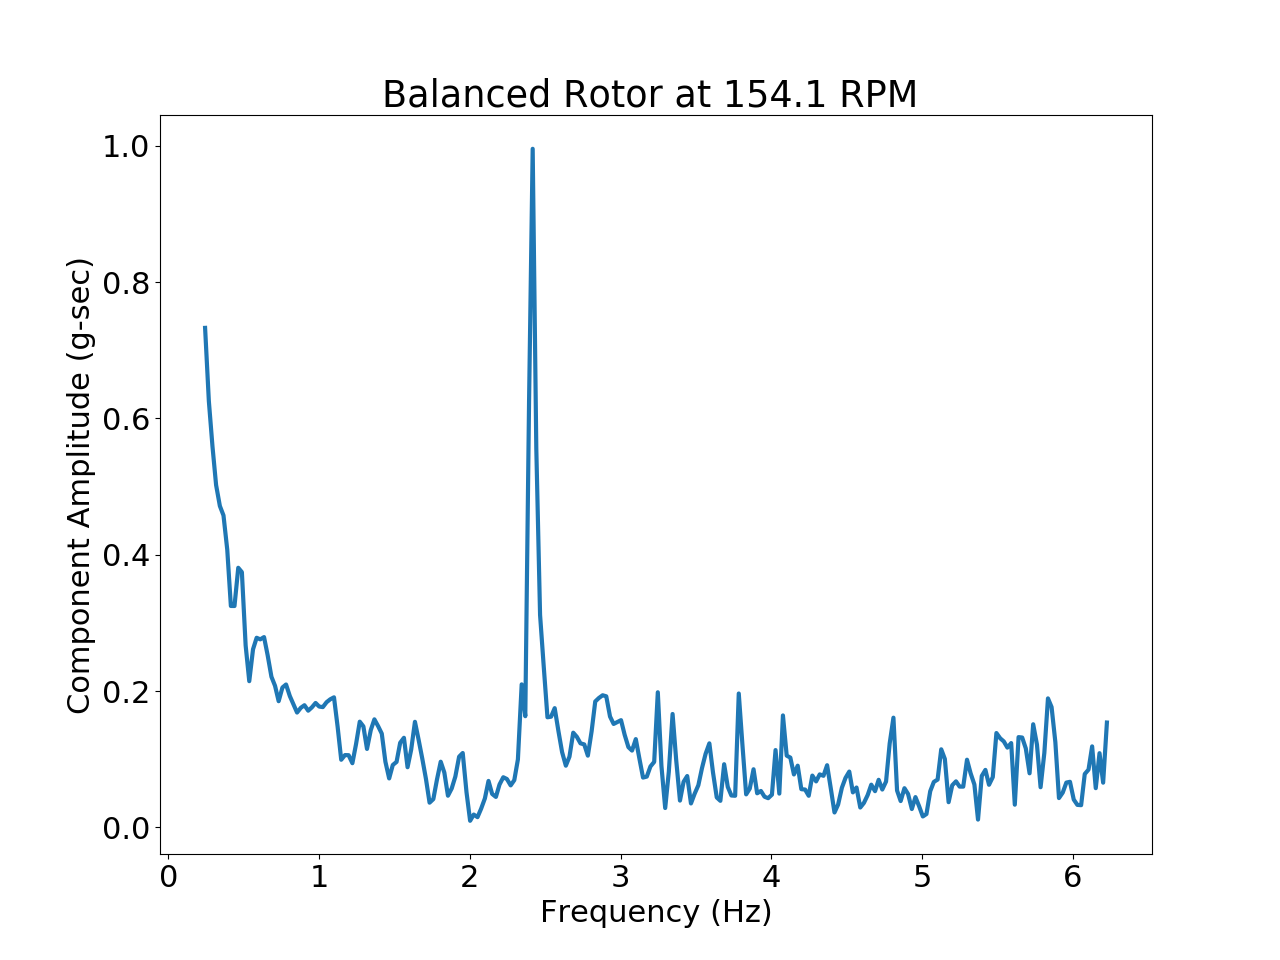
\includegraphics[scale=0.4]{single_DFT}
	\decoRule
	\caption{An example of a single DFT dataset from the LifeLine frequency data during a balanced rotor test.}
	\label{fig:single_DFT}
\end{figure}

\begin{figure}
	\centering
	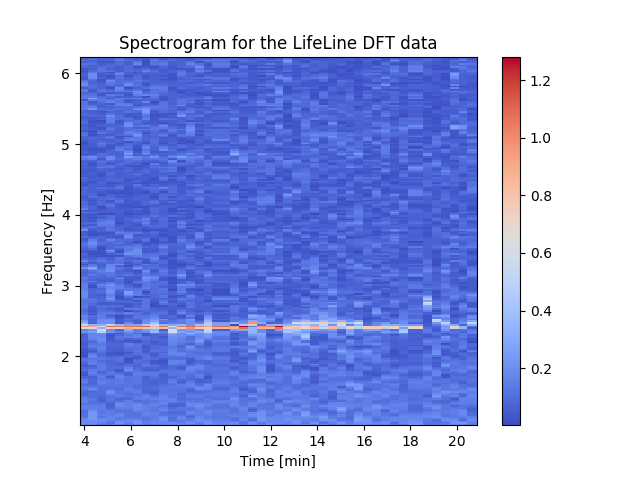
\includegraphics[scale=0.8]{LL_spectrogram}
	\decoRule
	\caption{A spectrogram showing the tower frequency domain data over the length of a single LifeLine file.}
	\label{fig:LL_spectrogram}
\end{figure}

The maximum frequency component and magnitude are plotted over time for the balanced rotor and shown in Figure \ref{fig:max_balanced_freq_mag}.  This data is very noisy and should be smoothed before applying any detection algorithm.

\todo{more explanation needed for the plots in this section.}

\begin{figure}
	\centering
	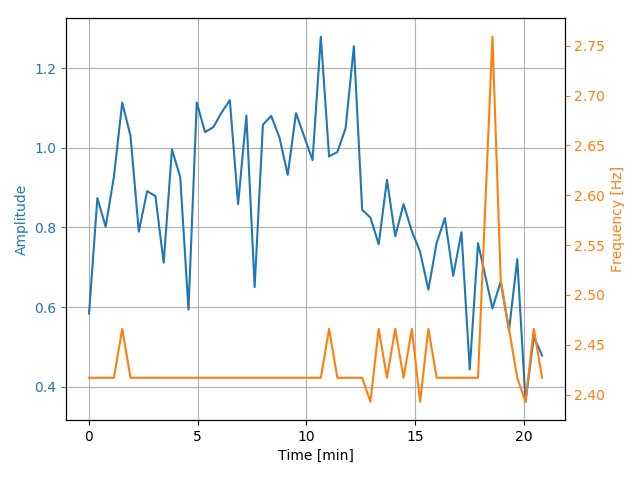
\includegraphics[scale=0.8]{max_balanced_freq_mag}
	\decoRule
	\caption{A plot of the raw maximum frequency/magnitude data of each DFT over time for a balanced rotor.  This data consists of a single point extracted from each DFT and plotted over time.}
	\label{fig:max_balanced_freq_mag}
\end{figure}


\subsection{Smoothing the data}
\subsubsection{Choosing the filter}
The filter choice is very important for noise reduction in a dataset.  Some of the common options are finite impulse response (FIR) filters, and infinite impulse response (IIR) filters, and the Savitzky-Golay (SG) filter.

The IIR filter is shown in Figure \ref{fig:freq_mag_IIR_filter}, which significantly smooths the data, but at the cost of some high frequency distortion.  An IIR filter uses past states in the output calculation, meaning an impulse input signal will affect the filter output forever (\textit{infinite} impulse response filter).  This results in a transfer function as follows:

\begin{equation}
	T(z) = \frac{b(z)}{a(z)}
\end{equation}

\begin{figure}
	\centering
	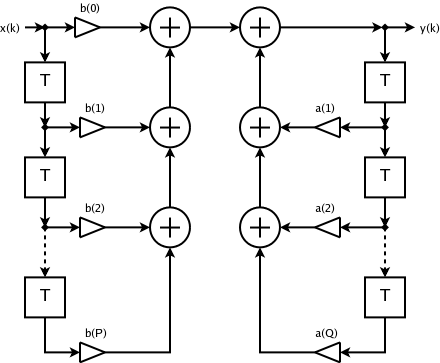
\includegraphics[scale=0.5]{IIR_block_diagram}
	\decoRule
	\caption{A block diagram of a standard IIR filter. \cite{wiki:IIR_block_diagram}}
	\label{fig:IIR_block_diagram}
\end{figure}

\begin{figure}
	\centering
	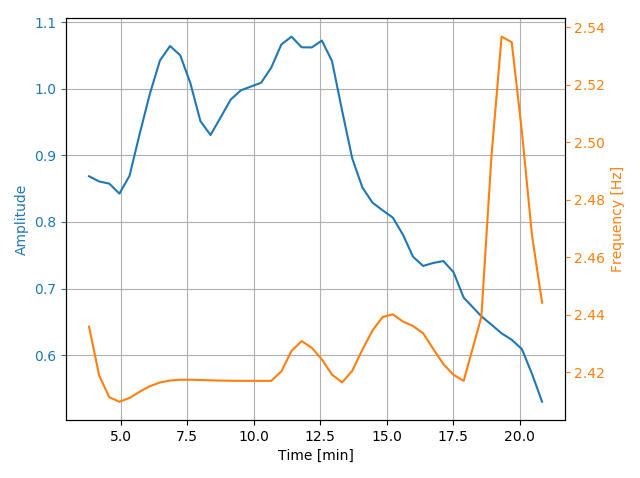
\includegraphics[scale=0.8]{freq_mag_IIR_filter}
	\decoRule
	\caption{The Figure \ref{fig:max_balanced_freq_mag} data with a Butterworth IIR filter applied.  The filter has an order of 2 and a normalized cutoff frequency of $0.1 \mathrm{\frac{rad}{sec}}$}
	\label{fig:freq_mag_IIR_filter}
\end{figure}

Another filter alternative is the FIR filter, which does not rely on past states to calculate the filter output.  This results in a finite response to an impulse input and a linear phase.  A common FIR filter that is used for smoothing data is a moving average (where all of the filter coefficients are identical).  To achieve a more customized filter for this data, a FIR filter is designed using the Window method, which designs a FIR filter using a specified window.  Figure \ref{fig:FIR_block_diagram} shows a block diagram of a FIR filter, and Figure \ref{fig:freq_mag_FIR_filter} shows the filter applied to the LifeLine data.  Because the past states are not used, the transfer function has a denominator of 1:

\begin{equation}
	T(z) = \frac{b(z)}{1}
\end{equation}

\begin{figure}
	\centering
	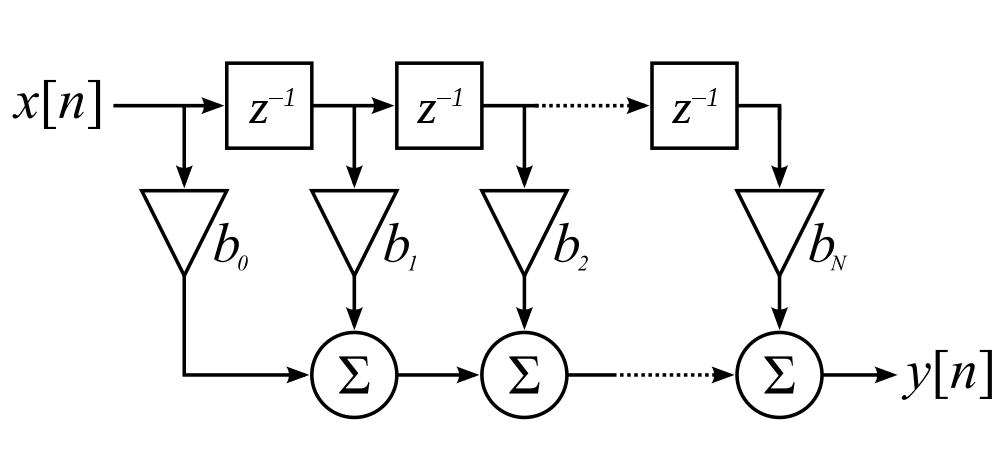
\includegraphics[scale=0.3]{FIR_block_diagram}
	\decoRule
	\caption{A block diagram of a standard FIR filter. \cite{wiki:FIR_block_diagram}}
	\label{fig:FIR_block_diagram}
\end{figure}

\begin{figure}
	\centering
	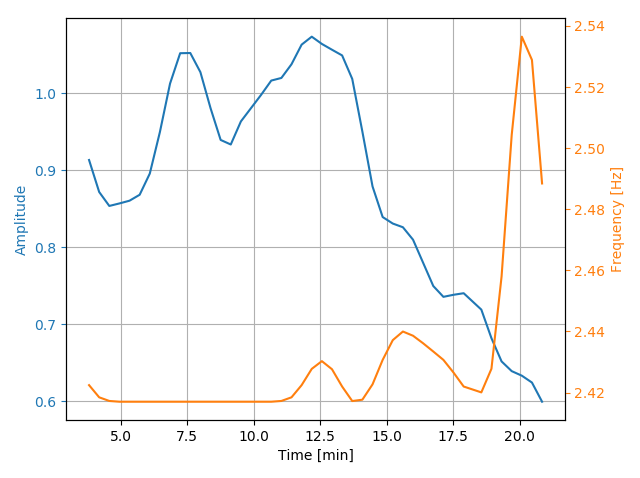
\includegraphics[scale=0.8]{freq_mag_FIR_filter}
	\decoRule
	\caption{The Figure \ref{fig:max_balanced_freq_mag} data with an Window FIR filter applied.  The filter has an order of 8 and a normalized cutoff frequency of $0.1 \mathrm{\frac{rad}{sec}}$.}
	\label{fig:freq_mag_FIR_filter}
\end{figure}

Another filter option for this data is the Savitzky-Golay (SG) filter, which increases the signal-to-noise ratio with out significantly distorting the signal.  The SG filter uses convolution to fit a polynomial on a sliding window to the data.  The output of this filter can be calculated using the following equation \cite{SG_filter}:

\begin{equation} \label{eq:SG_filter}
	Y_j = (\mat{C} \otimes y)_j = \sum_{i=-\frac{m-1}{2}}^{\frac{m-1}{2}} C_iy_{j+i}
\end{equation}

$C_i$ are the convolution coefficients ($m$ total coefficients), $y$ is the sampled data point, and $j$ is the index of the data point. 

The convolution coefficients can be selected from a table, but it is much more robust to calculate them prior to performing any filtering.  The convolution coefficients, $\mat{C}$, are calculated using a variable change.  The time vector for a given window, $\vec{x}$, is converted to $\vec{z}$ using the time step ($\Delta t$) with the following equation:

\begin{equation}
	z = \frac{\vec{x} - \bar{x}}{\Delta t}
\end{equation}

$\bar{x}$ is the time value at the central point of the window.  $\vec{z}$ is used to calculate the matrix $\mat{J}$, where each $i\mathrm{-th}$row of $\mat{J}$ has the values $1, z_i, z_i^2, z_i^3, ..., z_i^n$.  After $\mat{J}$ has been created, the convolution coefficients can be calculated as follows:

\begin{equation}
	\mat{C} = \left(\mat{J^TJ}\right)^{-1}\mat{J^T}
\end{equation}

The filtered data can then be calculated as the convolution of $\mat{C}$ and the unfiltered data (Equation \ref{eq:SG_filter}).

\subsubsection{Applying the filter}
A set of balanced data should have a constant maximum amplitude frequency with small amounts of high frequency signal, so A FIR or IIR filter is preferable over the SG filter.  Linear phase is not required for this filter, so an IIR filter design is chosen to achieve a lower filter order.  A Butterworth IIR filter, which is a type of signal processing filter designed to be flat in the passband, is ideal for this situation because the low frequency data is not distorted.

The filter parameters for this design are shown in Table \ref{t:IIR_filter_parameters}.  For a second order analog Butterworth filter, the following equation represents the generic transfer function  \cite{butter_filter_design}:

\begin{equation}
	H(s) = \frac{1}{s^2 + \sqrt{2} s + 1}
\end{equation}

This equation needs to be converted to the digital form, so a bilinear transformation needs to be applied, where:

\begin{equation}
	s = \cot({\omega_n)}\,\frac{1-z^{-1}}{1+z^{-1}}
\end{equation}

Using the filter parameters in Table \ref{t:IIR_filter_parameters}, the Butterworth IIR filter design transfer function is calculated to be:

\begin{equation} \label{eq:IIR_tf}
	H(z) = \frac{B(z)}{A(z)} = \frac{0.0675 + 0.1349z^{-1} + 0.0675z^{-2}}{1-1.143z^{-1} + 0.4128z^{-2}}
\end{equation}

Figure \ref{fig:IIR_filter_response} shows the filter response for the Butterworth IIR filter compared to a standard moving average filter with a window of 4 samples.  The IIR filter has a much stronger rejection of higher frequency components and only uses the last 2 samples (instead of the previous 4 samples that the moving average uses).  The moving average filter is essentially just a FIR filter with equal magnitude coefficients.

\begin{table}[]
\centering
\caption{IIR filter parameters}
\label{t:IIR_filter_parameters}
\vspace*{0.2in}
\begin{tabular}{|c|c|c|}
\rowcolor[HTML]{EFEFEF} 
\hline
\textbf{Variable} & \textbf{Value} & \textbf{Description} \\ \hline
$n$ & 2 & Filter order \\ \hline
$\omega_n$ & 0.2 & Normalized cutoff frequency \\ \hline
\end{tabular}
\end{table}


\begin{figure}
	\centering
	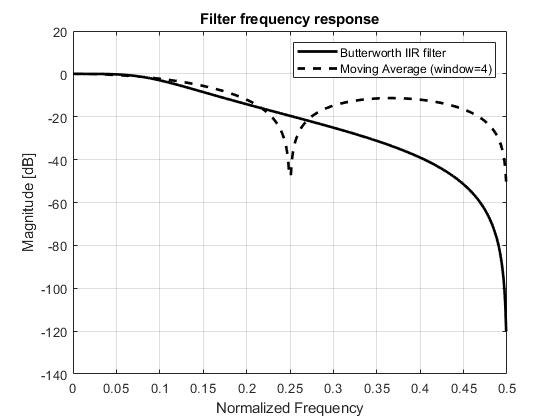
\includegraphics[scale=0.8]{IIR_filter_response}
	\decoRule
	\caption{The filter response of the Butterworth IIR filter (Equation \ref{eq:IIR_tf}) compared to a moving average filter with a window size of 4.  This figure was created in MATLAB with 2 simulated filter designs.}
	\label{fig:IIR_filter_response}
\end{figure}


%----------------------------------------------------------------------------------------
%	SECTION 2
%----------------------------------------------------------------------------------------
\section{Detecting an imbalance}

\todo{More explanation about the types of machine learning algorithms.  Explain the strengths and weaknesses of each method and include some background on machine learning.  Start with an explanation about the comparison between machine learning and linear regression.}

\subsection{Selecting a classification algorithm}
The crude and simple way to determine if there is an imbalance is to use a threshold criterion for the magnitude of the largest frequency component.  This method does not utilize the frequency values that correspond to each magnitude.  Since the rotor RPM is a range (not a constant value), it is likely that the magnitude will be slightly higher if the turbine is running faster and slightly lower if the turbine is running slower.  Additionally, the threshold method does not adapt the algorithm to patterns and new information gained from more data.

This is a standard "classification" problem, where the algorithm needs to classify the state of the turbine as \textit{balanced} or \textit{not balanced}.  With the modern availability of computational power, classification algorithms tend to fall under the "machine learning" category.  These algorithms consist of a model that adapts to training data in order to minimize the error.  A few of the common models include Logistic Regression (LR), Linear Discriminant Analysis (LDA), K-Neighbors Classifier (KNC), Decision Tree Classifier (DNC), Gaussian Naive Bayes (GNB), and Support Vector Classification (SVC).

The Logistic Regression model is commonly used to estimate discrete values (0/1 or false/true) and uses the logistic curve equation as the probability model.  The Linear Discriminant Analysis model address many of the shortcomings of the Logistic Regression model, such as multi-class classification and a higher stability.  Because the turbine classification problem only has 2 classes, this model is not likely to be the most optimal.

The K-Neighbors Classifier model is one of the simplest models, but can be the most accurate and powerful when dealing with fairly small datasets.  This model essentially "memorizes" the training data and plots the points in $n$-dimensional space.  The classification of the new point is calculated based on the distances between the new point and the training points.  This model is likely to be an accurate algorithm for the turbine problem.

Decision Tree Classification relies on the ability to split the data set into binary categories and subcategories, where the algorithm can follow yes/no decisions to lead to the correct class.

The Gaussian Naive Bayes model is a statistics based model that modifies a prior belief bell curve based on the training data.  This is a statistical method of classifying data where the data set statistics are constantly updated with new data (as opposed to static models, such as mean, median, and standard deviation classification).

The Support Vector Classification model creates a $n$-dimensional space where the training data points are divided by a clear gap that is as wide as possible.

To compare the listed classification models against each other, the accuracy of each model is plotted using the same training and test data.  Figure \ref{fig:algorithm_comparison} shows that the K-Neighbors Classification algorithm has one of the highest mean accuracy ratings with the smallest variation is accuracy scores.  This is also the simplest to design and implement, which makes it an ideal choice for the imbalance detection algorithm that may need to run on a microprocessor attached to the turbine tower.

\begin{figure}
	\centering
	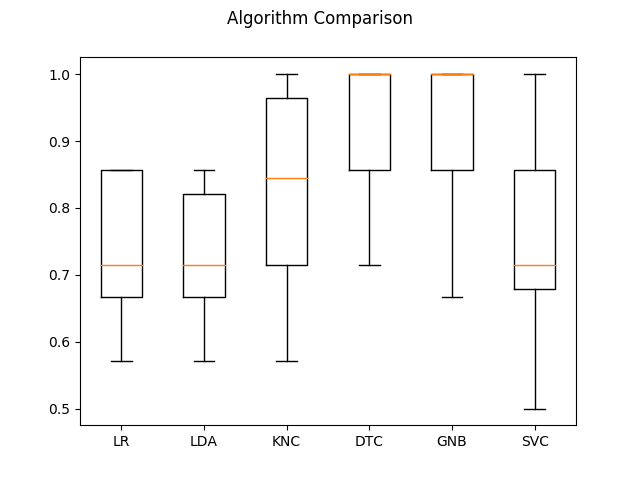
\includegraphics[scale=0.8]{algorithm_comparison}
	\decoRule
	\caption{A statistical comparison of different classification algorithms.  The algorithms compared are: Logistic Regression (LR), Linear Discriminant Analysis (LDA), K-Neighbors Classifier (KNC), Decision Tree Classifier (DNC), Gaussian Naive Bayes (GNB), and Support Vector Classification (SVC). \todo{Add axis label}}
	\label{fig:algorithm_comparison}
\end{figure}

\subsection{Applying the K-Neighbors Classification Algorithm}
\subsubsection{About the algorithm}
The K-Neighbors Classifier (also known as the K-Nearest Neighbors Classifier or K-NN Classifier) is a type of "lazy learning" \cite{k_NN_algorithm}, which means it memorizes the training data and uses it to calculate the test data classification.  This results in a very short training time, but a longer calculation time curing the classification process.


The K-NN algorithm uses a "majority voting" method where the Euclidian distance between all the training data points and the test data is calculated.  This model assumes there is a relatively equal amount of balanced rotor experimental data and imbalanced experimental rotor data, which means the sample weighting can be uniform.  If there is a much higher frequency class (for example, much more balanced experimental data), this class will tend to dominate the calculations regardless of the actual class of the test data.

The number of neighbors, $k$, is chosen to be 5 for this algorithm (using trial and error).  A larger value of $k$ will reduce the classification noise, but the boundaries are much more general and not as tuned to the training data.  A lower value of $k$ will match the model very closely to the training data, but may add noise into the classification process.

The Euclidean distance is simply the distance between the data points.  This equation is shown below:

\begin{equation}
	d = \sqrt{\sum{\left(x_{i,a}-x_{j,a}\right)^2}}
\end{equation}

\subsubsection{Algorithm Results}
To apply the algorithm, the data is converted into short lists containing a maximum amplitude, a corresponding frequency value, and the known class. For this test, there are 55 experimental DFT results for a balanced rotor and 55 experimental DFT results for an imbalanced rotor.  Applying the algorithm on raw DFT data produces the classification boundary plot shown in Figure \ref{fig:classification_boundaries_no_filter}.  Using unfiltered data is slightly faster (there is no filter lag), but the accuracy is significantly reduces.  It is much more accurate to filter the data first, if the lag is an acceptable consequence.  The unfiltered data produces an accuracy of about 86 percent with a confusion matrix:

\todo{Explain what a confusion matrix is.}

\begin{equation}
C_{confusion} = 
\begin{bmatrix}
	13 & 0 \\
	3 & 6
\end{bmatrix}
\end{equation}

\begin{figure}
	\centering
	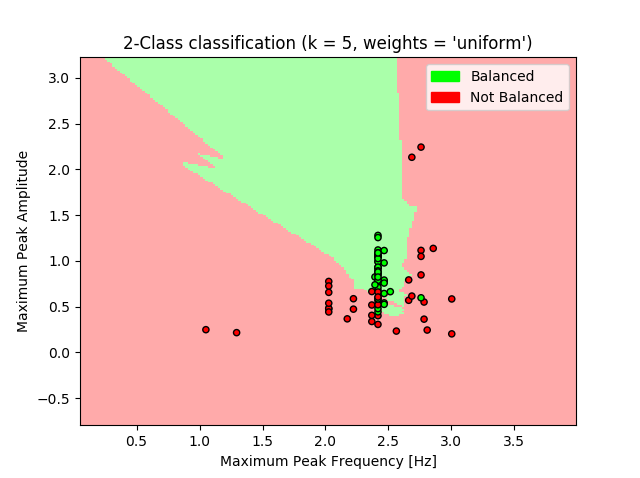
\includegraphics[scale=0.8]{classification_boundaries_no_filter}
	\decoRule
	\caption{The classification boundaries for test and training data that is not filtered.}
	\label{fig:classification_boundaries_no_filter}
\end{figure}

Figure \ref{fig:classification_boundaries_filter} shows the classification boundaries with data filtered using an IIR filter.  A clear trend can be seen in this data, with distinct class boundaries.  This produces an accuracy of 94 percent with a confusion matrix:

\begin{equation}
C_{confusion,filtered} = 
\begin{bmatrix}
	6 & 1 \\
	0 & 11
\end{bmatrix}
\end{equation}

The filtered data produces a much more accurate detection model because much of the time-dependent noise is suppressed.  It is difficult to draw conclusive results from these test results, since there are only 55 sets of balanced and imbalanced data.  80 percent of this data is used to train the detection algorithm, while the remaining 20 percent is used to perform the verification testing shown in the confusion matrices and accuracy results.

Both the amplitude and frequency values are important in detecting an imbalance in the turbine rotor.  An imbalance will cause overall higher acceleration amplitudes, but will also cause a larger variation in rotor speeds.  As shown in Figure  \ref{fig:classification_boundaries_filter}, the imbalanced data has large variations in both the maximum amplitude and frequency of the LifeLine DFT data.  When there is an imbalance in the rotor, the closed-loop transfer function of the changes, causing error in the tuned rotor speed controller parameters.  This causes some instability in the controller that is identified by the DFT results of the LifeLine module.

Additionally, this algorithm can also be made more robust by looking for 10 or more positive imbalance detections in a row before flagging an alert.  This will remove any false positives that could shut the turbine down unintentionally.

\begin{figure}
	\centering
	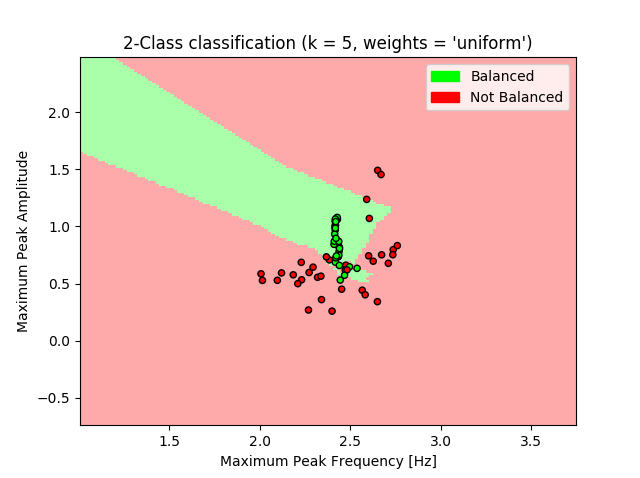
\includegraphics[scale=0.8]{classification_boundaries_filter}
	\decoRule
	\caption{The classification boundaries for test and training data that \textit{is} filtered.}
	\label{fig:classification_boundaries_filter}
\end{figure}


%----------------------------------------------------------------------------------------
%	SECTION 3
%----------------------------------------------------------------------------------------
\section{Analyzing the Detection Algorithm}
\subsection{Using Different Parameters}
The main parameters to tune for the detection model are $k$ and the weighting.  In the KNN algorithm, the classification decision is based on the weighted vote from $k$ neighboring samples.  This means that a larger $k$ value will include more data in each decision, but may be lest accurate.  A smaller $k$ value will create tight classification boundaries, but could be prone to over-fitting.  Figure \ref{fig:classification_k_20_uniform} and Figure \ref{fig:classification_k_2_uniform} show the effect of changing the $k$ value on the classification boundaries.

\begin{figure}
	\centering
	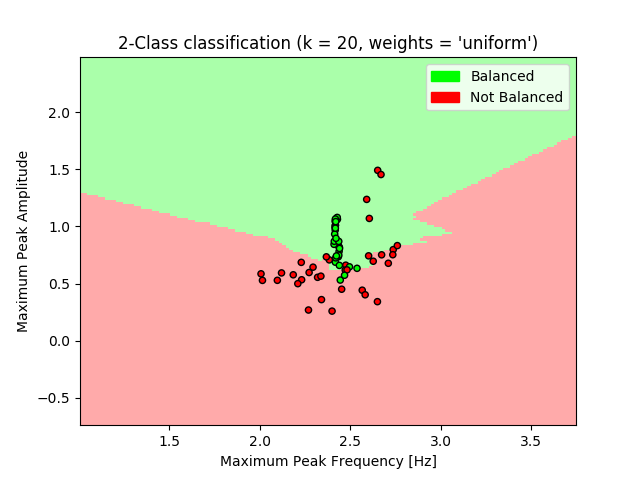
\includegraphics[scale=0.8]{classification_k_20_uniform}
	\decoRule
	\caption{The classification boundaries with $k=20$ and uniform weighting.}
	\label{fig:classification_k_20_uniform}
\end{figure}

\begin{figure}
	\centering
	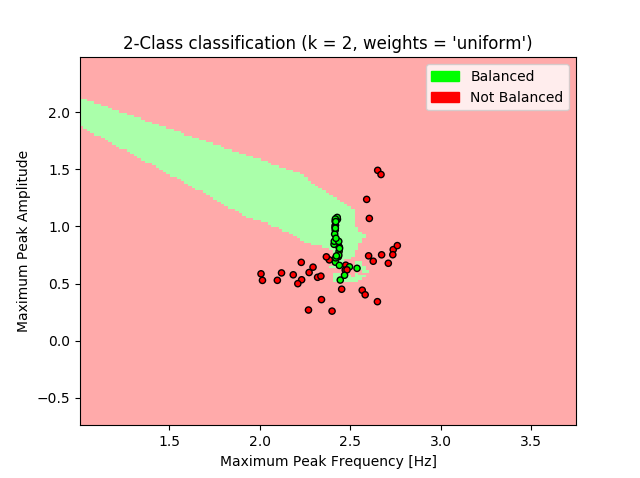
\includegraphics[scale=0.8]{classification_k_2_uniform}
	\decoRule
	\caption{The classification boundaries with $k=2$ and uniform weighting.}
	\label{fig:classification_k_2_uniform}
\end{figure}

\subsection{Potential Problems}
One of the biggest problems with the KNN classification algorithm is the computational cost.  Because this is a "memory-based" model, the training data is essentially locked in memory and used to classify any new inputs.  By changing the model, the computational cost can be reduced; however, these are much more complicated to implement and not always as accurate.

Additionally, the IIR filter has a fairly significant and nonlinear delay that increases near DC frequency components.  Faster filters can be used at the cost of accuracy because they will produce more noise or a more distorted signal.  For this application, it seems like accuracy is more important than speed, and the IIR filter parameters were designed around this idea.

This detection algorithm is best developed with real experimental data, which means it requires actual data before it is of any use.  If a sufficient enough model is developed, the model can produce the test data to train the algorithm instead of collecting it in the field; however, this is likely to be less accurate.

\subsection{Future Changes}

\todo{Add a section about algorithm scalability and switching to a model-based machine learning algorithm (like a neural network) if many training sets are acquired.}

One of the significant benefits with this algorithm is the flexibility.  It is very easy to add more data to improve the imbalance detection.  For example, in addition to peak frequency and magnitude, the wind speed and generator power can be included as parameters to improve the model.  With enough variables and experimental data, the model will become more accurate and robust (although it is difficult to visualize the classification space with orders higher than 2).

In addition, the entire frequency spectrum can be used as an input to the algorithm (instead of just using the peak values), but the model becomes much more complex.  With a large amount of experimental data, the KNN model might need to be changed to a less computationally intensive model, such as a neural network.

Just using a classification algorithm on raw data isn't always useful.  It is very important to properly choose a data processing methods, such as the IIR filter used in this paper.  Selecting the filter is just as important as choosing the model for this type of data.

\todo{Add a section with conclusions, recommendations for future work, and methods for algorithm improvement.  Add code to a public repository.}











